\documentclass[a4paper]{article}

\usepackage[french]{babel}
\usepackage[utf8]{inputenc}
\usepackage[T1]{fontenc}
\usepackage{fullpage}
\usepackage{hyperref}
\usepackage{graphicx}
\usepackage{float}

\author{Titouan \bsc{Christophe}}
\title{Synthèse de bases de données}
\date{\today}

\begin{document}
\maketitle
\tableofcontents

\section{Modèle entité-relation}
Un schéma conceptuel des données, pas forcément implémenté de cette façon.
Selon le contexte, désigne la classe (modèle) ou l'objet (l'instance).

\subsection{Entité}
\begin{figure}[H]
    \center
    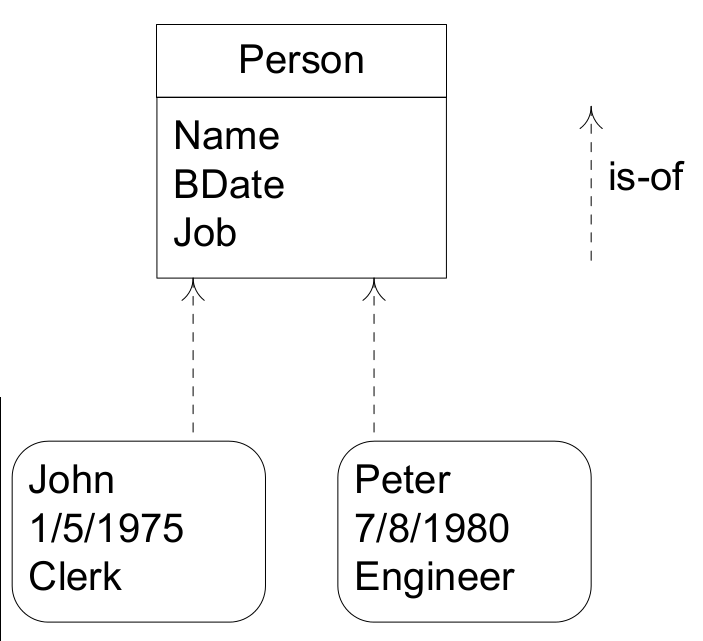
\includegraphics[width=.3\textwidth]{fig/entity.png}
    \caption{Une entité}
\end{figure}

\subsubsection{Attributs}
Les entités ont des attributs, qui ont une cardinalité minimale et maximale

\paragraph{Attributs multivalués}
Attributs dont la cardinalité maximale est supérieure à 1.
Exemple: \texttt{Person.degrees}

\paragraph{Attributs dérivés}
Attributs calculés à partir d'autres attributs, pas stockés dans la base de donnée.
Exemple: à partir du champ \texttt{Person.birth}, on peu déduire \texttt{Person.age}

\paragraph{Attributs composites}
Attributs formés par l'aggrégation de plusieurs autres attributs.
Exemple: \texttt{Person.Adress = \{Street, City, State, Zipcode, Country\}}

\paragraph{Clefs ou identificateurs}
Attributs ou ensemble d'attributs d'une entité dont les valeurs sont uniques
(déterminent une et une seule entité). On les met en évidence dans un schéma
entité-relation en les soulignant, en ajoutant un symbole \textit{clef} à côté,
ou en les mettant dans une section à part dans la boîte de l'entité.
\subparagraph{Clefs primaires}
Seule l'une des clefs peut être soulignée, et est l'identifiant d'un objet pour
cette entité.

\subsection{Relation}
\begin{figure}[H]
    \center
    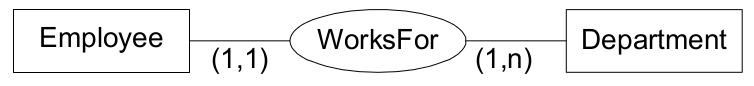
\includegraphics[width=.4\textwidth]{fig/relation.png}
    \caption{\label{fig:relation}Une relation One-to-many}
\end{figure}
\begin{figure}[H]
    \center
    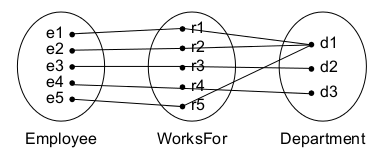
\includegraphics[width=.3\textwidth]{fig/relation-ensembliste.png}
    \caption{Vue ensembliste de la relation à la Figure \ref{fig:relation}}
\end{figure}
\begin{itemize}
  \item On doit spécifier la multiplicité minimale et maximale pour chaque pair de la relation
  \item La relation porte un nom (souvent lié au sens et à la sémantique de la relation)
  \item Chaque entité à un rôle dans la relation
  \item Une relation peut contenir des attributs
  \item L'arité ($x$-ary) d'une relation, ou son \textbf{degré}, indique le nombre d'entités participant à la relation
  \item \textbf{One-to-one}, \textbf{one-to-many} ou \textbf{many-to-many} pour les relations binaires
\end{itemize}

On peut noter qu'il n'y a pas de différence fondamentale entre un attribut et une relation,
juste une question de point de vue. On préfèrera une relation si on souhaite mettre en évidence
les liens entre plusieurs objets, et un attribut quand c'est une propriété comme un autre.

\subsubsection{Relation n-aire}
Une relation n-aire implique plus que 2 entités différentes.

\begin{figure}[H]
    \center
    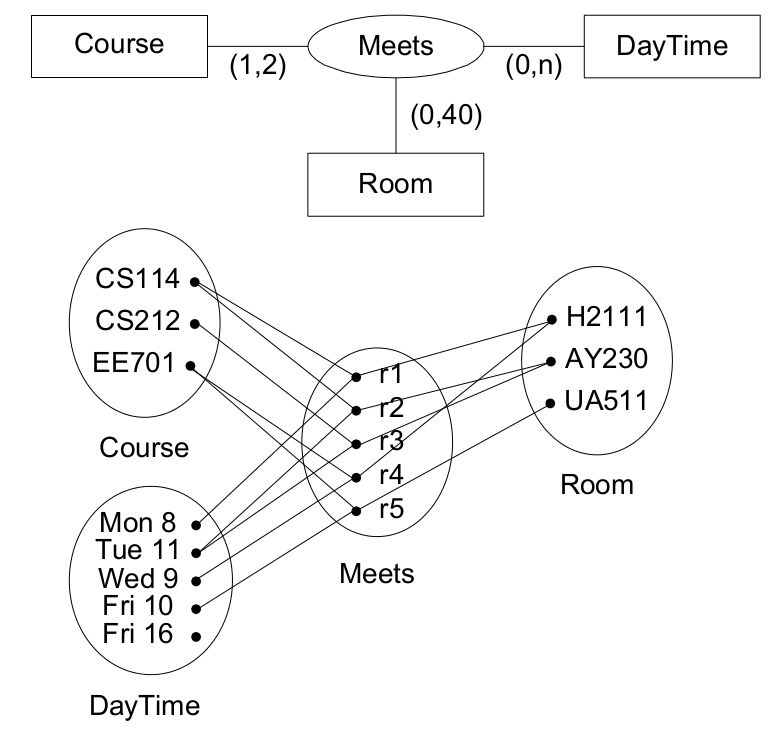
\includegraphics[width=.4\textwidth]{fig/relation-naire.png}
    \caption{Une relation ternaire et sa vue ensembliste}
\end{figure}

\subsubsection{Transformation des relation n-aires en binaires}
Les relations obtenues après transformation \textbf{par projection} contiennent moins d'information
que la relation initiale. Par exemple, dans la Figure \ref{fig:relation-naire-projection},
on voit que la relation ternaire indique qu'un fournisseur délivre un produit pour un projet,
tandis que les relations binaires indiquent uniquement qu'un fournisseur délivre un produit,
qu'un projet utilise un produit, et qu'un projet utilise un fournisseur.

\paragraph{Projection}
On crée une relation pour chaque paire possible de la relation
\begin{figure}[H]
    \center
    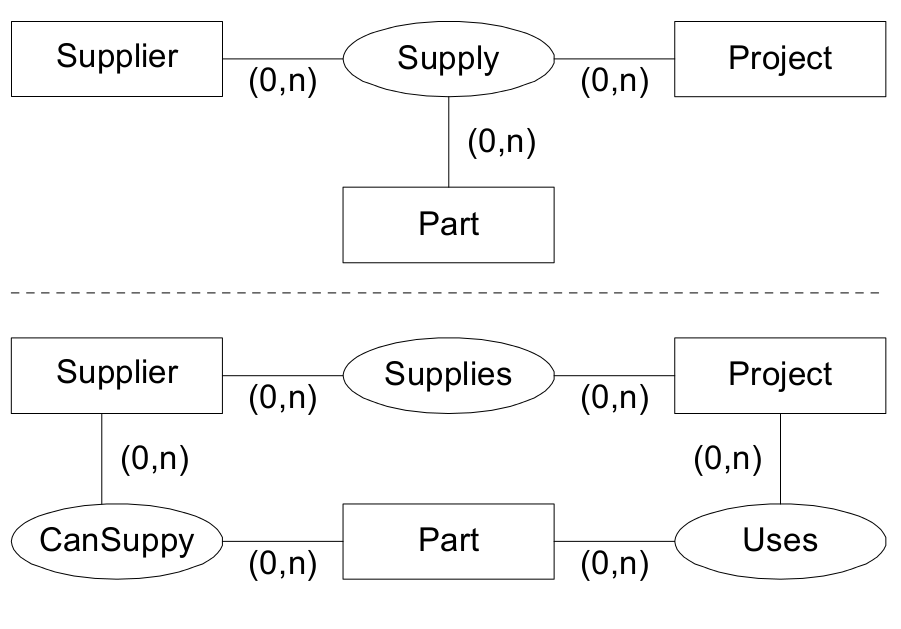
\includegraphics[width=.4\textwidth]{fig/relation-naire-projection.png}
    \caption{\label{fig:relation-naire-projection}Projection d'une relation ternaire}
\end{figure}

\paragraph{Insertion}
On transforme la relation en entité, et on la lie par des relations binaires à
toutes les entités de la relation initiale.
\begin{figure}[H]
    \center
    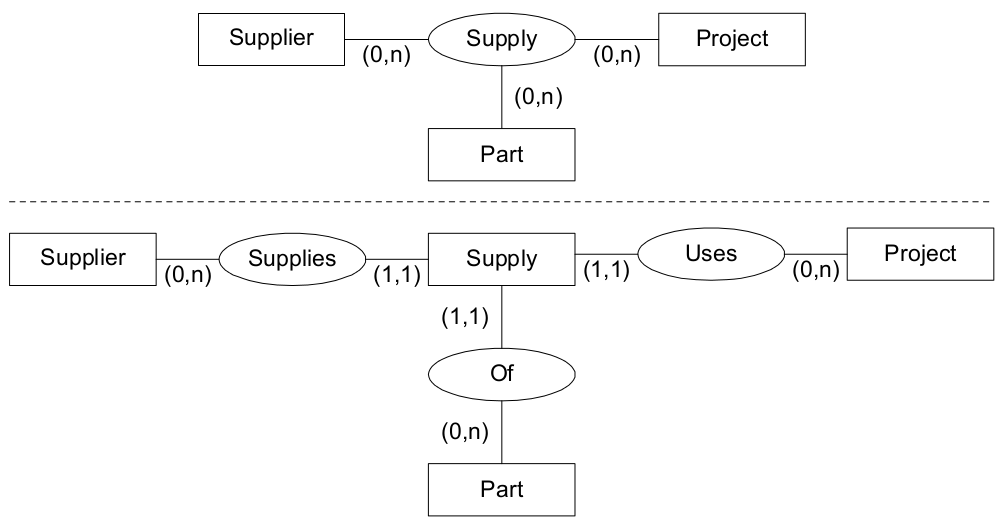
\includegraphics[width=.6\textwidth]{fig/relation-naire-insertion.png}
    \caption{Transformation par insertion}
\end{figure}

\subsection{Entités faibles}
Une entité faible n'a aucune clef ne dépendant que de ses propres attributs, et
a donc une \textbf{clef partielle} qui la distingue des autres entités ayant la
même clef étrangère.

\paragraph{Intérêt des entités faibles}
\begin{itemize}
  \item Suppression des attributs redondants
  \item Réduction des relation n-aires en relations binaires par la méthode d'insertion
  \item Héritage et polymorphisme (ajout des attributs des entités filles dans des entités faibles)
\end{itemize}

\subsection{Relation génériques}
\'Equivalent des design pattern pour les relations. Elle dénotent la nature d'une
relation sur un schéma entité-relation.

\subsubsection{Classification}
Utilisée lorsqu'on instancie un objet. Exemple: on a une liste de destinations
au départ d'un aéroport (classe), et les vols chaque jour vers ces destinations (instance).

\subsubsection{Généralisation (héritage)}
Relation spéciale entre une ou plusieurs sous-entités et une superentité, plus abstraite.

\begin{figure}[H]
    \center
    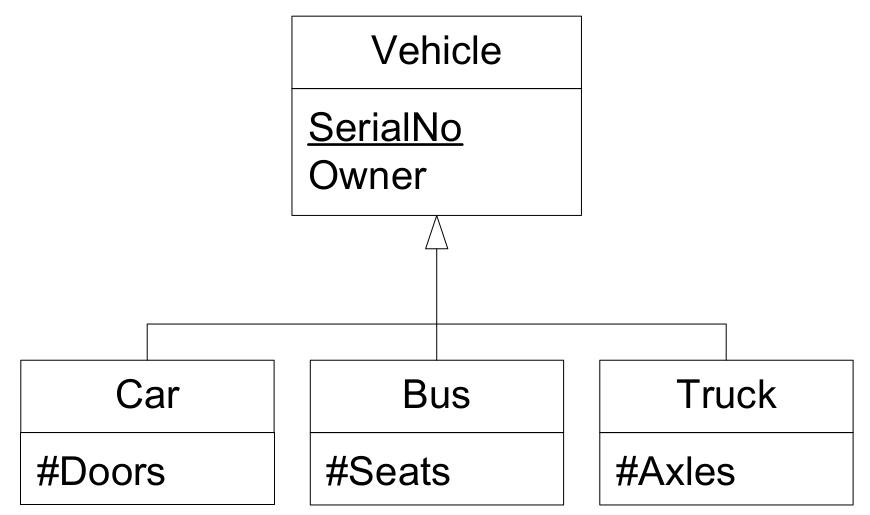
\includegraphics[width=.3\textwidth]{fig/generalisation.png}
    \caption{Généralisation}
\end{figure}

\paragraph{Différent types de recouvrements}
\begin{itemize}
  \item \textbf{Partiel} ou \textbf{Total}: les entité filles ont-elles des attributs de la superentité ?
  \item \textbf{Exclusif} ou \textbf{Recouvrant (overlapping)}: les entités filles partagent-elles des attributs ?
  \item La spécialisation peut être déterminée par un prédicat (ex: \texttt{Person.age < 18 -> Child})
  \item Les clefs sont héritées, et de nouvelles clefs peuvent être définies par les entités filles
\end{itemize}
\begin{figure}[H]
    \center
    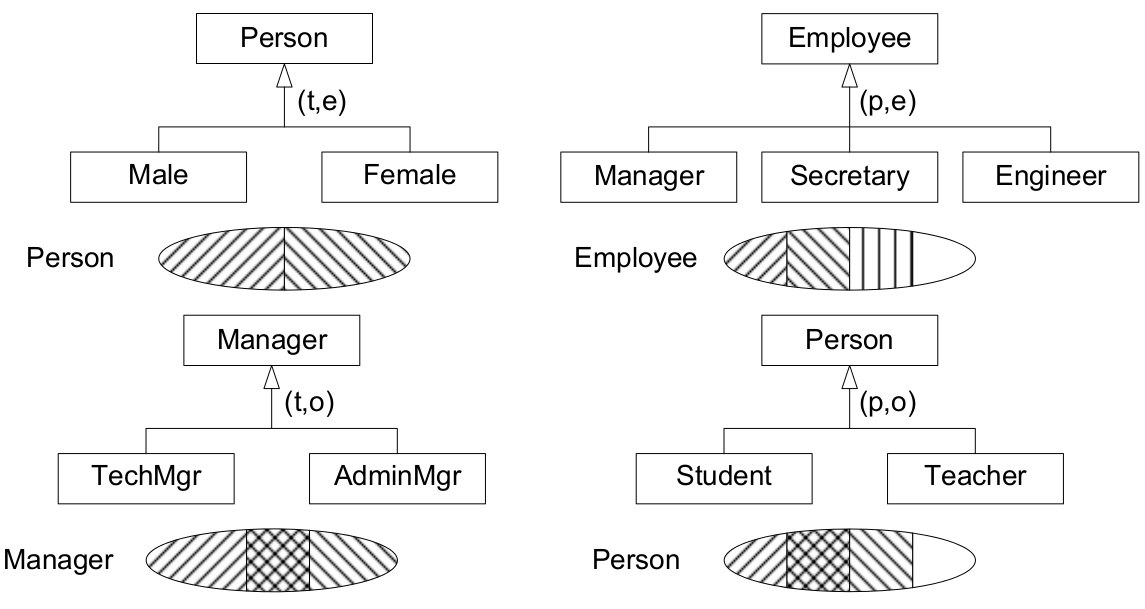
\includegraphics[width=.6\textwidth]{fig/generalisation-cov.png}
    \caption{Combinaisons de recouvrements partiels et totaux, exclusifs et recouvrants}
\end{figure}

Les contraintes de recouvrement influencent l'implémentation.


%%%%%%%%%%%%%%%%%%%%%%%%%%%%%%%%%%%%%%%%%%%%%%%%%%%%%%%

\section{Modèle relationnel}
Données structurées en tables bidimensionnels de valeurs simples. Les lignes
sont aussi appelées tuples, et les colonnes attributs.
Les relations sont des tables avec des restrictions:
\begin{itemize}
  \item L'ordre des lignes n'a pas d'importance
  \item L'ordre des colonnes n'a pas d'importance
  \item La table a au moins une clef (pas de lignes en double exemplaire)
\end{itemize}
La relation peut être vue comme un prédicat, par exemple comme un ensemble de propriétés.

Les bases de données sont des collections de relations, mais ne pas oublier que
les structures relationnelles sont plus riches que les tables, et que le modèle de 
données ne définit pas que les structures de données, mais aussi des opérations
pour les manipuler.

\subsection{Schéma}
On parle du schéma pour décrire le modèle des données (le nom des colonnes).

\begin{figure}[H]
    \center
    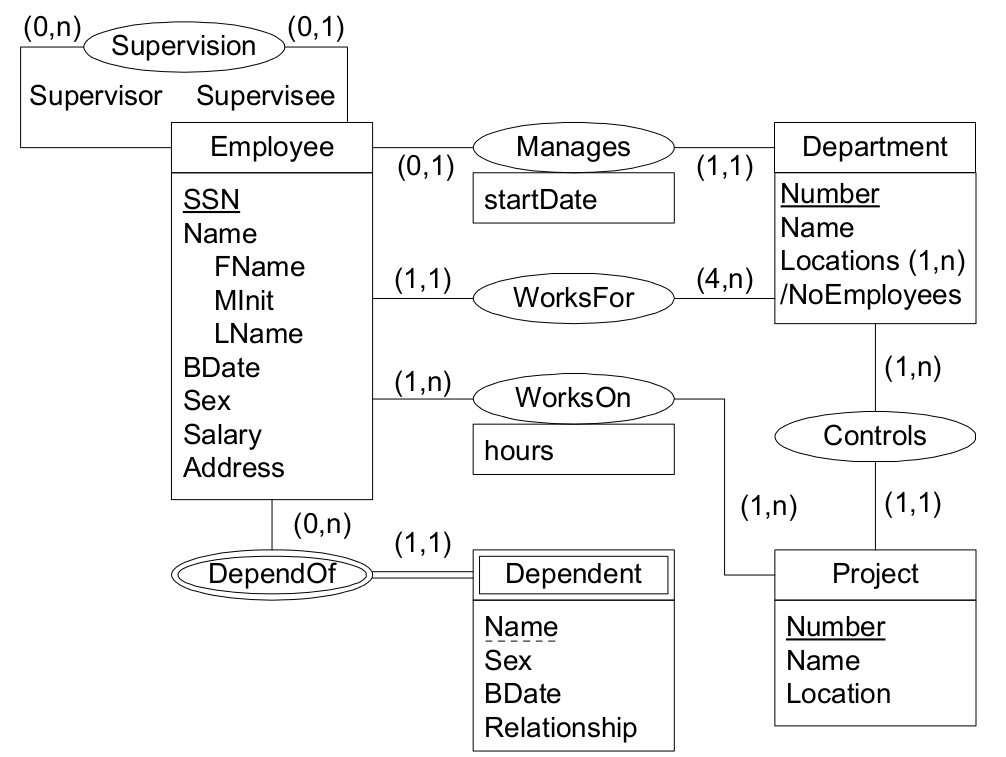
\includegraphics[width=.5\textwidth]{fig/relmodel-er.png}
    \caption{\label{fig:relmodel-er}Un modèle Entité-Relation}
\end{figure}
\begin{figure}[H]
    \center
    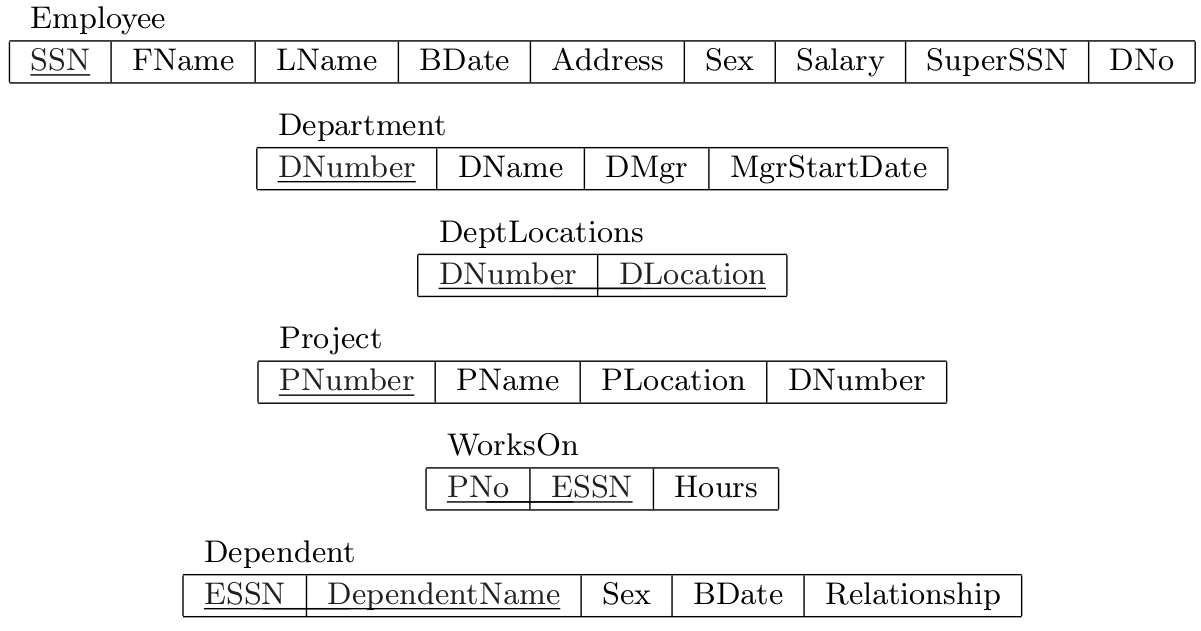
\includegraphics[width=.7\textwidth]{fig/relmodel-tuples.png}
    \caption{Les tuples correspondant au schéma Figure \ref{fig:relmodel-er}}
\end{figure}

Lors de la traduction du modèle entité-relation en modèle relationnel, on voit
que toutes les relations ne sont pas matérialisées par une table (par exemple,
un \texttt{Department} contient directement la clef de son manager et sa date d'entrée en service),
et que certaines tables ne sont pas modélisées par une entité ou une relation, mais
par un attribut multivalué (\texttt{Department.location})

\subsection{Relations}
Le schéma auquel on adjoint les valeurs donnent une relation. Plus formellement, on a
\begin{equation}
  R(A_1:D_1, ~ ... ~ , A_n:D_n)
\end{equation}
Où $R$ est la relation, les $D_i$ sont un ensemble de valeurs atomiques appelées le \textbf{domaine},
les attributs $A_i$ sont distincts dans la relation. $A_i : D_i$ dénote la structure de la relation.
\'Etant donné un tuple\footnote{un ensemble de paires attribut:valeur} $\{A_1: d_1, ~...~, A_n: d_n\}$, on a la valeur relationelle
\begin{equation}
  \rho \subseteq \{\{A_1:d_1, ~...~, A_n:d_n\} \mid d_i \in D_i\}
\end{equation}

Le domaine définit la comparabilité des valeurs: des attributs ne peuvent être comparés
que s'ils sont sur le même domaine. On peut voir le domaine comme des types définis par
l'utilisateur.

\subsection{Clefs de relation}

\paragraph{Une super-clef} désigne un ou plusieurs attributs qui, ensemble, identifient
un et un seul tuple.

\paragraph{Une clef} est une super-clef minimale (si un seul des attributs est
enlevé de la super-clef minimale, elle perd sa propriété d'identification unique).
Généralement, une relation a plusieurs clefs, qu'on appelle aussi clefs candidates.

\paragraph{La clef primaire} est une clef choisie parmi les clefs candidates comme étant
la seule qu'on utilisera pour identifier un tuple.

\subsection{Contraintes relationnelles}
Les contraintes font parties du schéma, et spécifient des prescriptions ou
assertions sur les données. Elles permettent de garantir l'intégrité des données.

\subsubsection{Intégrité référentielle}
\'Etant donné une contrainte relationelle sur $R_1$ et $R_2$, $\exists$ un attribut
$A_2$ de $R_2$ tq. $A_2$ a le même domaine que la clef primaire de $R_1$ et toute
valeur de $A_2$ dans un tuple de $R_2$ apparaît comme clef primaire dans le tuple
de $R_1$. On appelle $A_2$ une clef étrangère. $A_2$ n'est pas forcément une clef
de $R_2$

\begin{figure}[H]
    \center
    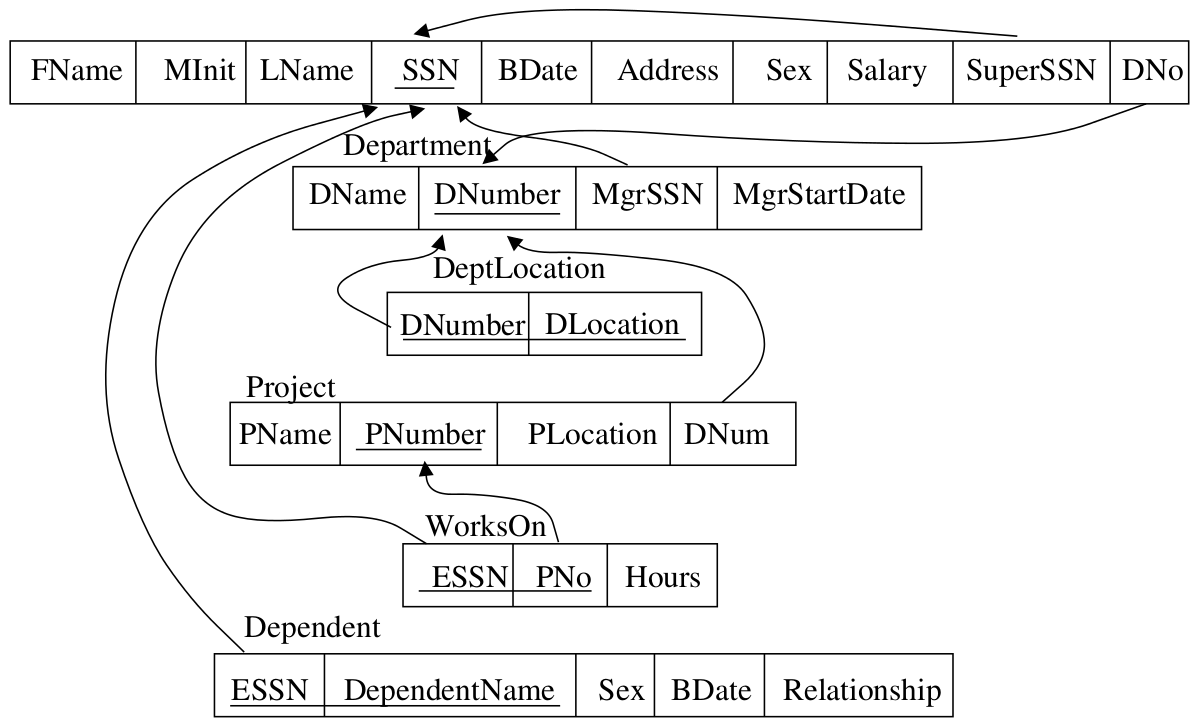
\includegraphics[width=.7\textwidth]{fig/integrite-rel.png}
    \caption{Intégrité référentielle du schéma Figure \ref{fig:relmodel-er}}
\end{figure}

\subsubsection{Contraintes transitionelles}
On impose une contrainte sur la mise à jour de la valeur d'un attribut (exemple:
une personne ne peut pas changer de sexe, un salaire ne peut qu'augmenter...)

\subsubsection{Contraintes structurelles}
\paragraph{Intégrité de la clef}
Toute relation a une clef primaire et éventuellement d'autres clefs

\paragraph{Intégrité de domaine}
Les valeurs des attributs doivent correspondre au domaine (type et opérations permises)

\paragraph{Intégrité de l'entité}
Les clefs primaires ne sont pas nulles

\paragraph{Intégrité de colonne}
Une contrainte spécifique imposée sur une colonne (ex: la date est supérieure à l'an 2000)

\paragraph{Intégrité de ligne}
Contrainte sur un tuple en particulier (ex: la date de retraite doit être postérieure
à la date de premier emploi).

\subsubsection{Suppression d'un tuple}
Quand la suppression d'un tuple viole une contrainte d'intégrité référentielle,
il faut exécuter une des actions suivantes :
\begin{itemize}
  \item rejeter la suppression
  \item propager la suppression aux tuples qui référencent le tuple supprimé
  \item nullifier les valeurs d'attributs des tuples qui référencent le tuple supprimé,
  sauf si ces attributs font partie de la clé primaire
\end{itemize}

\subsection{Implémentation dans les DBMS}
Un DBMS a donc:
\paragraph{Un langage de définition des données (DDL)} permettant de créer le schéma
\paragraph{Un langage de manipulation des données (DML)} pour accéder aux valeurs.
Par exemple, l'algèbre relationelle ou le calcul tuple. SQM redéfinit les opérations
correspondantes et définit quelques extensions (les fonctions d'aggrégation par exemple).
\paragraph{Des opération d'altération} permettant de modifier ou supprimer des valeurs et des schémas.
Ces opérations doivent tenir compte des contraintes (en émettant une erreur si l'une d'elle est violée par exemple).
\paragraph{Des vues (éventuellement)} décrivant des relations dérivées
(relations inférées à partir d'autres). Elles peuvent être enregistrées sur le
disque (snapshots), mais ça peut poser des problème de redondance.

\subsection{Traduction depuis un schéma E-R}
\subsubsection{Suppression des généralisations}
\paragraph{Tout dans la superentité}
Tous les champs de toutes les entités filles sont dans la superentité. Les attributs
inexistants pour une entité fille sont nuls. On rajoute un champ pour déterminer
le type d'enfant du tuple (dans l'exemple ci-dessous, \texttt{Rank}).\\

Il faut parfois également rajouter des contraintes (ci-dessous, par exemple :
seulement les étudiants avec \texttt{Rank == GradStud} ont un advisor).
\subparagraph{Avantage}
Facile et rapide à mettre en place, toujours utilisable.
\subparagraph{Inconvénients}
Gaspillage d'espace (beaucoup d'attributs nuls), les opérations sur les entités
filles doivent être exprimée sur la superentit (programme plus complexe).
\begin{figure}[H]
    \center
    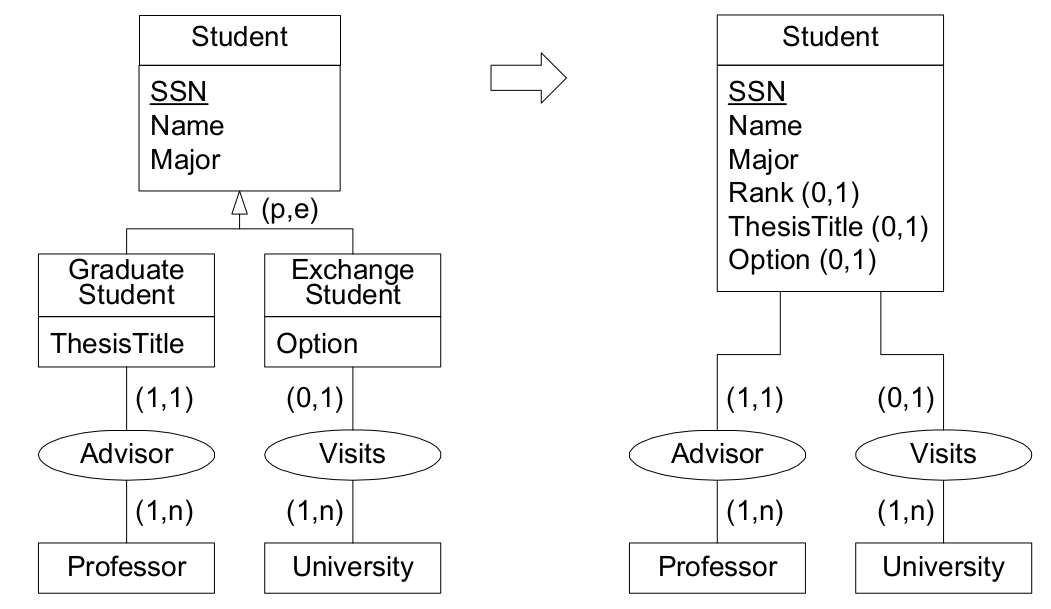
\includegraphics[width=.7\textwidth]{fig/er2rm-1.png}
\end{figure}

\paragraph{Garder les entités filles}
On ne crée que les entités feuilles dans l'arbre d'héritage, il n'existe pas de
table pour la superentité. Chaque entité fille contient ses attributs propres et
ceux de sa superentité. \textbf{Il faut garantir avec une contrainte que les
clefs sont uniques parmis l'ensemble de toutes les entités filles.}
\subparagraph{Inconvénients}
Beaucoup d'attribut redondants et de relations, rendant les applications plus complexes.
Utilisable avec les relations totales-exclusives uniquement.
\begin{figure}[H]
    \center
    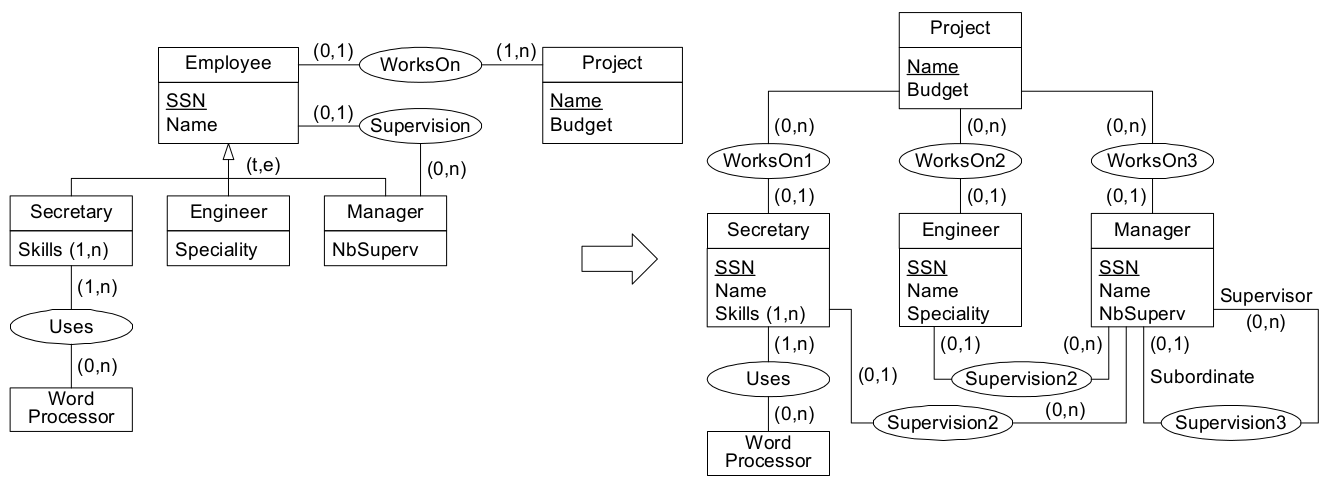
\includegraphics[width=.9\textwidth]{fig/er2rm-2.png}
\end{figure}

\paragraph{Transformation en relations}
Une table pour chaque entité. On crée une relation one-to-one entre une entité
et sa superentité. Les filles sont des entités faibles.
\subparagraph{Inconvénients}
Redondance (beaucoup de relations signifient la même chose), il faut des contraintes
pour exprimer le type de généralisation (recouvrement). Les opération deviennent plus
complexes (en O(n) de la profondeur de l'arbre d'héritage).
\begin{figure}[H]
    \center
    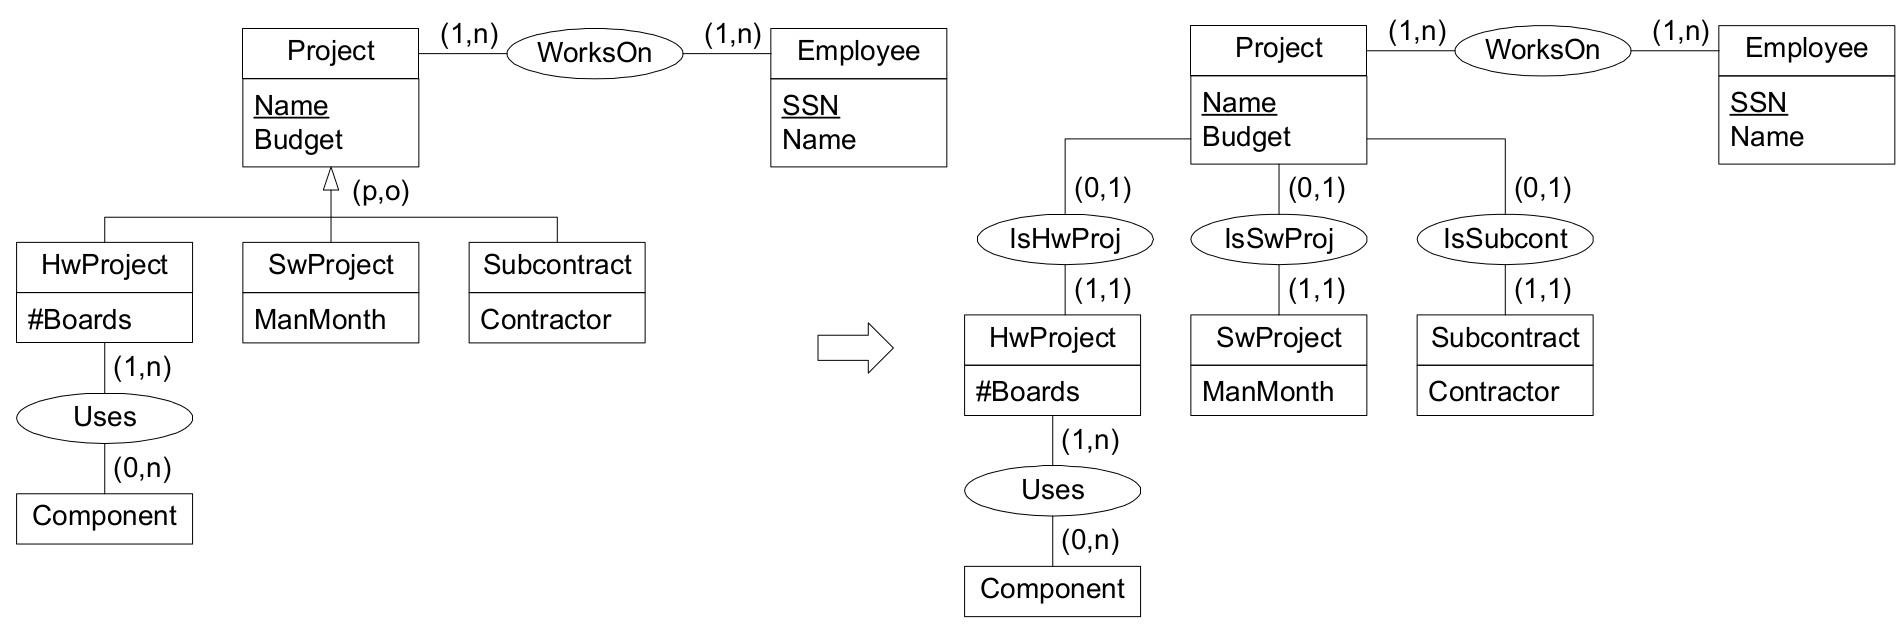
\includegraphics[width=.9\textwidth]{fig/er2rm-3.png}
\end{figure}

\paragraph{Traduction des entités et relations en tables} les attributs deviennent
des colonnes, faire attention aux attributs multivalués, les entité fortes et faibles.
Les relations doivent se traduire par des 


%%%%%%%%%%%%%%%%%%%%%%%%%%%%%%%%%%%%%%%%%%%%%%%%%%

\section{Algèbre relationnel}

%%%%%%%%%%%%%%%%%%%%%%%%%%%%%%%%%%%%%%%%%%%%%%%%%%

\section{Calcul tuple/relationnel}


\end{document}